\section*{Desarrollo}
En esta secci\'on se podran observar los pasos para el diseño del filtro y el detalle de los c\'alculos emplados para lograr la salida requerida, junto con las prubeas y respuestas en frecuencia pedidas.\\

%---------------------------------------------------------------%

\subsection*{Problema a resolver}
El filtro a diseñar vino dado por la siguiente imagen de un diagrama de \textit{Bode}. \\
\begin{figure}[H]
	\centering
	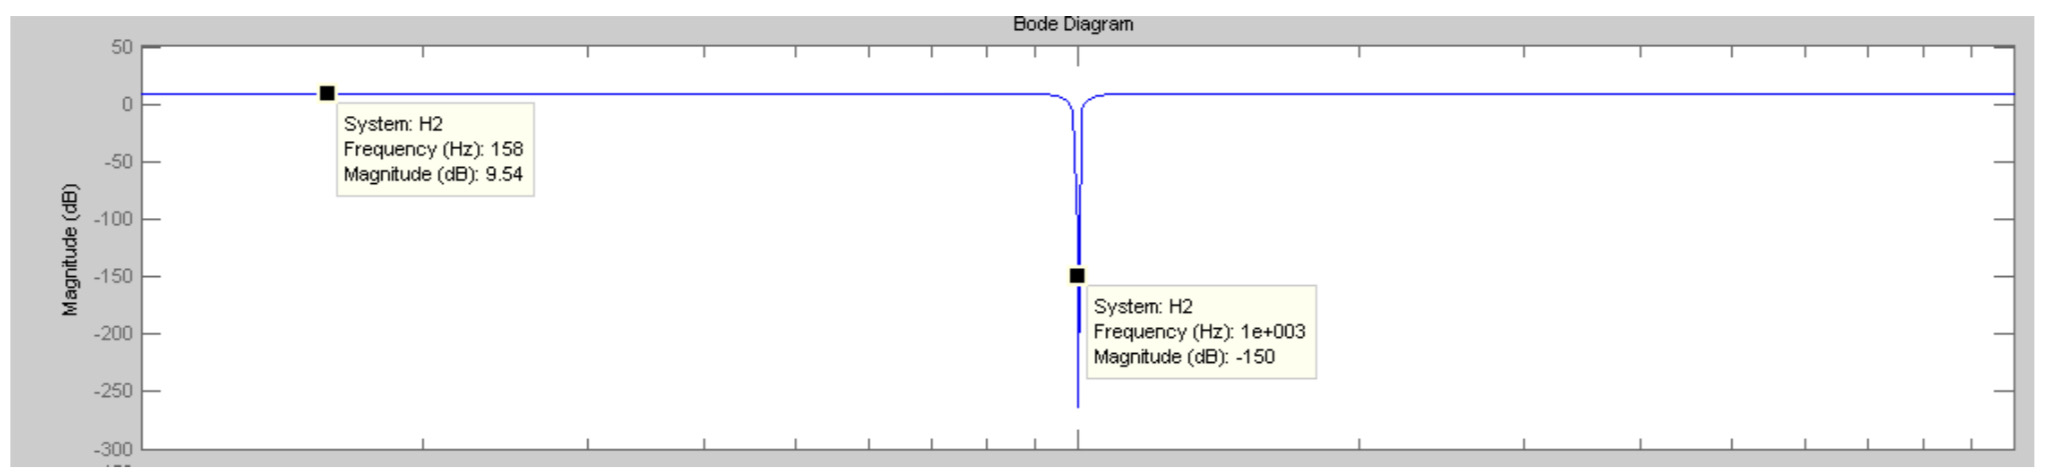
\includegraphics[width=15cm]{imagenes/consigna}
	\caption{Consigna del filtro a diseñar}
	\label{img:consigna}
\end{figure}

Se observa que es un filtro del tipo \textit{Notch} o \textit{Elimina banda} para la frecuencia de $1\kHz$ y tambien que para el resto de las frecuencias, posee un nivel de amplifiaci\'on de $9.54\dB$.

\subsection*{Diseño del filtro}
Se identificaron los par\'ametros de la transferencia del filtro a partir de la forma de Bode vista en clase.\\

\begin{equation}
  H(s)=H_0\ \frac{s^2 + \omega_0 ^2}{s^2 +s \frac{\omega_0}{Q} +\omega_0}
\end{equation}
De la  consigna se ve que la frecuencia de corte es $f_0 = 1\kHz$, por lo que $\omega_0 = 2\pi f_0= 2000\pi$. En $\omega_0$ se encuentra el polo doble de la transferencia.
Luego se eligi\'o un coeficiente de selectividad $Q > \frac{1}{\sqrt 2}$ (para que funcione como elimina banda) pero no tan grande que luego el circuito pueda correr riesgo de comportarse como oscilador. Se eligi\'o $Q= 2.5$ en funci\'on de los valores de resistencia y capacitor convenientes para el circuito.
Luego, del dato del primer punto medido en la consigna, se despej\'o el valor de $H_0$ de la siguiente expresi\'on
\begin{equation}
  H_0^x = 20 \log (H_0^{dB})
\end{equation}
Viendo en la cosigna que los valores de amplificacion fuera de la frecuencia de corte es $9.54 \dB$ se obtiene $H_0 = 3 $.

%---------------------------------------------------------------%

\subsection*{Circuito}
Se utiliz\'o el siguiente circuito visto en clase
%TODO: insertar circuito  notch sin ampli al final

\begin{figure}[h]
\begin{center}
\begin{circuitikz} [american,scale=0.4,transform shape]
\draw
% primeras resistencias
(0,0) node[left] {$v_i$} to [short,o-] (1,0)

		to[R, l=$R$] (4,0) -- (5,0) 
		
		to[R,l=$R$] (7,0) -- (8,0)
%capacitores de abajo y los R y C que bajan
(5,0)		to[C,*-,l=$C$,-*] (5,-6)
(1,0)	-- (1,-2) to [C,l=$C/2$] (4,-2) -- (5,-2) to[C, l=$C/2$] (7,-2) -- (7,0) 
(3.5,-2) to[R,*-,l=$R/2$] (3.5,-6)to (8,-6)

%op de arriba  y pote
(9,0.49) node[op amp] (opamp1) {}
(opamp1) node[]{U1}
(opamp1.-) -- (7.8,2) -- (10.2,2)--(opamp1.out) 
(opamp1.out) -- (11,0.49) --(11,-2) to [potentiometer,l=$R_0$, n=POT, mirror] (11,-9) node[ground]

%op de salida
%(13,0) node[op amp,yscale=-1] (opamp3) {}
%(opamp3) node[]{U3}
%(opamp1.out) -- (opamp3.+)
(opamp1.out) to [short,-o] (12,0.5) node[right] {$v_o$}
%(opamp3.-) -- (11.8,-1.5)	to [R,l=$R$] (14.2,-1.5)--  (opamp3.out)
%(11.8,-1.5) to [R,l=$R/2$] (11.8,-4) node[ground]

%op de abajo 
(9,-6)  node[op amp, rotate=180] (opamp2) {}
(opamp2) node[]{U2}
(opamp2.-) -- (10.2,-8) -- (7.8	,-8) -- (opamp2.out)
(opamp2.+) to (POT.wiper)
;
\end{circuitikz}
\end{center}
\caption{Circuito de filtro Notch}
\end{figure}	

Aplicando el metodo de \textit{Nodos} se llega a la siguiente transferencia
\begin{equation}
  H(s) = \frac{s^2 \frac{RC}{2}^2+1}{s^2 \frac{RC}{2}^2+s \frac{RC}{2} 4(1-k)+1}
\end{equation}
	Notando que $\omega_0 = \frac{2}{RC}$, se elig\'o  un valor de capacitor tal que la resistencias se encuente entre $1\kohm$ y $1\megohm$. Tambien se consider\'o  que al elegir un valor comercial que diste del valor teorico, va a existir un error. Considerando esto, se eligi\'o $C= 10 \nF$ y $R= 33 \kohm$, \'este valor de resistencia es el que menos error presenta del valor teorico ($R_{teo}=31.83 \kohm$).\\
	Hasta ahora, el circuito funciona como elimina banda para la frecuencia de $1\kHz$, pero no amplifica en $9.54 \dB$ el resto de las frecuencias. Para ello, se empleo un amplificador en configuraci\'on \textit{No inversor} a la salida del filtro. Resultando en el siguiente circuito.\\
\begin{figure}[h]
\begin{center}
\begin{circuitikz} [american,scale=0.4,transform shape]
\draw
% primeras resistencias
(0,0) node[left] {$v_i$} to [short,o-] (1,0)

		to[R, l=$R$] (4,0) -- (5,0) 
		
		to[R,l=$R$] (7,0) -- (8,0)
%capacitores de abajo y los R y C que bajan
(5,0)		to[C,*-,l=$C$,-*] (5,-6)
(1,0)	-- (1,-2) to [C,l=$C/2$] (4,-2) -- (5,-2) to[C, l=$C/2$] (7,-2) -- (7,0) 
(3.5,-2) to[R,*-,l=$R/2$] (3.5,-6)to (8,-6)

%op de arriba  y pote
(9,0.49) node[op amp] (opamp1) {}
(opamp1) node[]{U1}
(opamp1.-) -- (7.8,2) -- (10.2,2)--(opamp1.out) 
(opamp1.out) -- (11,0.49) --(11,-2) to [potentiometer,l=$R_0$, n=POT, mirror] (11,-9) node[ground]

%op de salida
(13,0) node[op amp,yscale=-1] (opamp3) {}
(opamp3) node[]{U3}
(opamp1.out) -- (opamp3.+)
(opamp3.out) to [short,-o] (15,0) node[right] {$v_o$}
(opamp3.-) -- (11.8,-1.5)	to [R,l=$R$] (14.2,-1.5)--  (opamp3.out)
(11.8,-1.5) to [R,l=$R/2$] (11.8,-4) node[ground]

%op de abajo 
(9,-6)  node[op amp, rotate=180] (opamp2) {}
(opamp2) node[]{U2}
(opamp2.-) -- (10.2,-8) -- (7.8	,-8) -- (opamp2.out)
(opamp2.+) to (POT.wiper)
;
\end{circuitikz}
\end{center}
\caption{Circuito de filtro Notch y amplificador}
\end{figure}	
\\

Donde $R_0$ es un preset de $100 \kohm$
Para los valores de $R$ y $C$ elegidos, resulta la siguiente transferencia teorica

\begin{equation}
	H(s)=\frac{3s^2+12\times10^6 \pi^2}{s^2+s\ 800\pi+ 4\times10^6 \pi^2}
\end{equation}

\subsection*{Diagramas de Bode}
Para la transferencia hallada, se realizaron los diagramas de Bode en el software \texttt{Matlab} de calculo num\'erico. Definiendo a $s$  como una variable de transferencia y con la funcio\'on \textit{bode()} se obtuvo la siguiente figura\\
%\pagebreak
\begin{figure}[h]
	\centering
	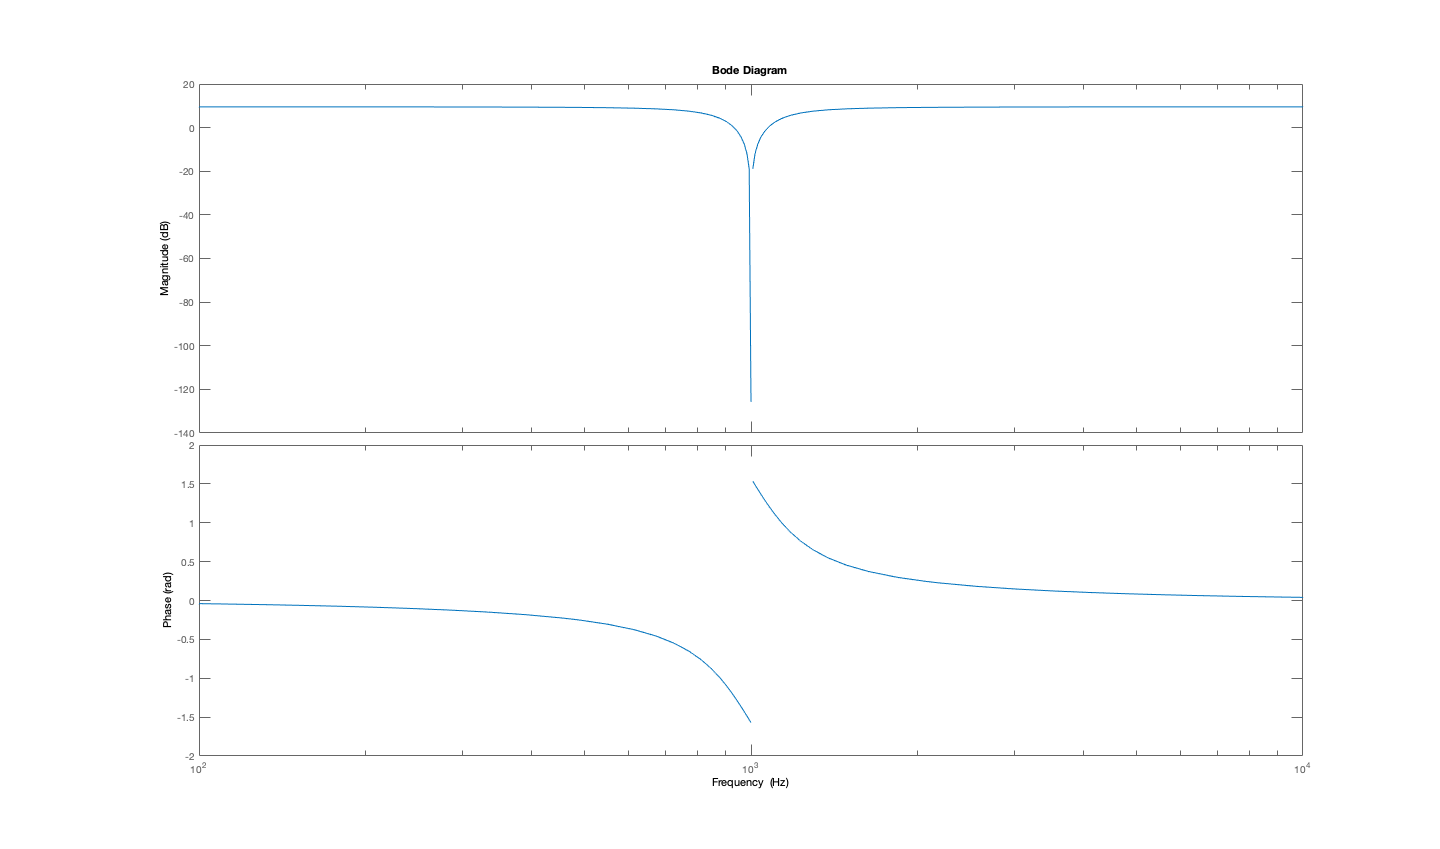
\includegraphics[width=9cm]{imagenes/BodeTeorico}	\caption{Diagrama de Bode teorico en Matlab}
\end{figure}

Se puede apreciar el comportamiento de \textit{elimina-banda} y tambien que est\'a aplicado a la frecuencia correcta. Luego viendo el nivel de amplificacion para el resto de las frecuencias, se mide un nivel de $9.45 \dB$, lo cu\'al coincide con el esperado.
%---------------------------------------------------------------%
\subsection*{Respuesta del filtro teorico a distintas señales}
Luego del diagrama de Bode, se realizaron graficos donde se muestran qu\'e salida tiene el filtro dada una señal de entrada como: \textit{escal\'on}, \textit{impulso}, \textit{senoidal}, \textit{cuadrada}.\\
Para la respuesta a señal senoidal, se  eligieron 3 frecuencias  acordes a las caracteristicas del filtro, $f_1=  10 \Hz$, $f_2= 1\kHz$ y $f_3 = 1 \MHz$.\\
Para la respuesta a la señal cuadrada, se eligieron tambien,  3 frecuencias acordes, $f_4 = 100 \Hz$, $f_5 = 1\kHz$, $f_6 = 100 \kHz$.
Se lograron los siguientes resultados.\\

\begin{figure}[hbt]
	\centering
	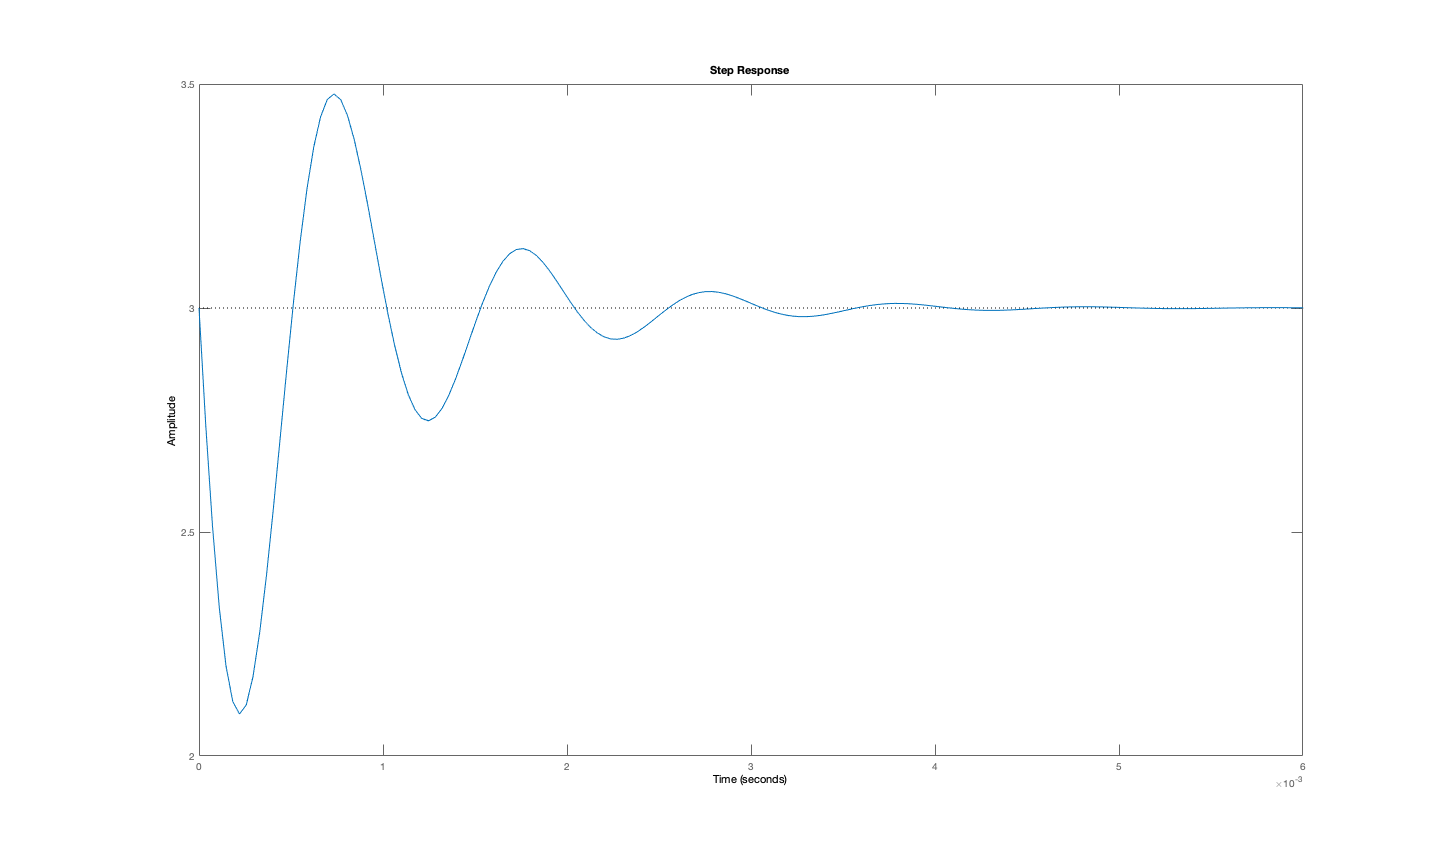
\includegraphics[width=9cm]{imagenes/stepTeorico}
	\caption{Respuesta al escal\'on.}
\end{figure}
Se puede observar que se logra un nivel de tensi\'on estable cerca de los $6 \ms$, adem\'as, se ve que el valor al que estabiliza es $3 \V$, que es acorde a la  amplificacion de $3\ veces$ o $9.54 \dB$.\\

\begin{figure}[hbt]
	\centering
	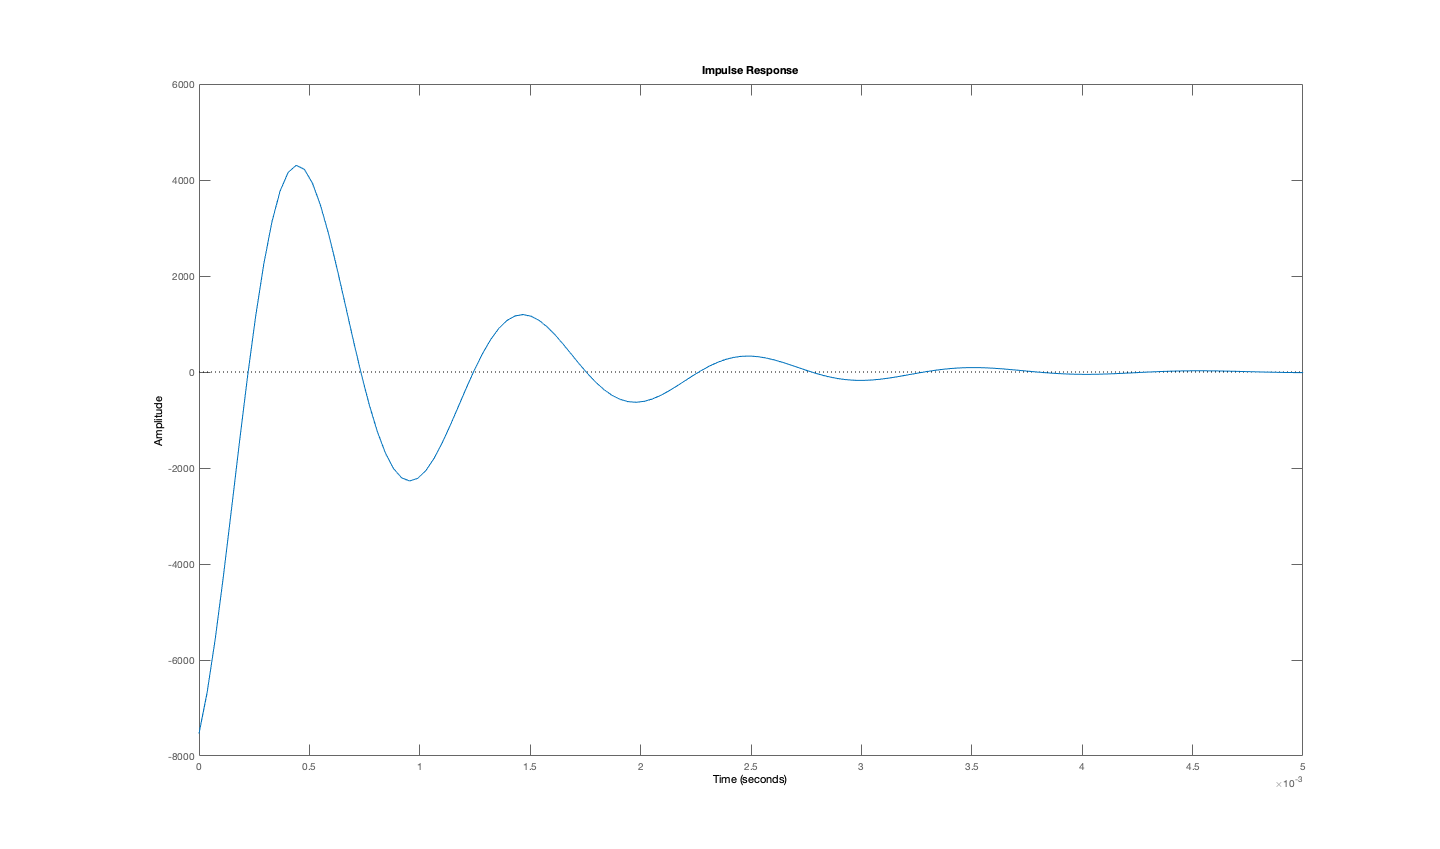
\includegraphics[width=8cm]{imagenes/impulseTeorico}	\caption{Respuesta al impulso.}
\end{figure}
Aqui se observa que existe mucha mas variaci\'on de tensi\'on en el transitorio hasta los $3 \V$, que se alcanzan en $5 \ms$.\\

\begin{figure}[hbt]
	\centering
	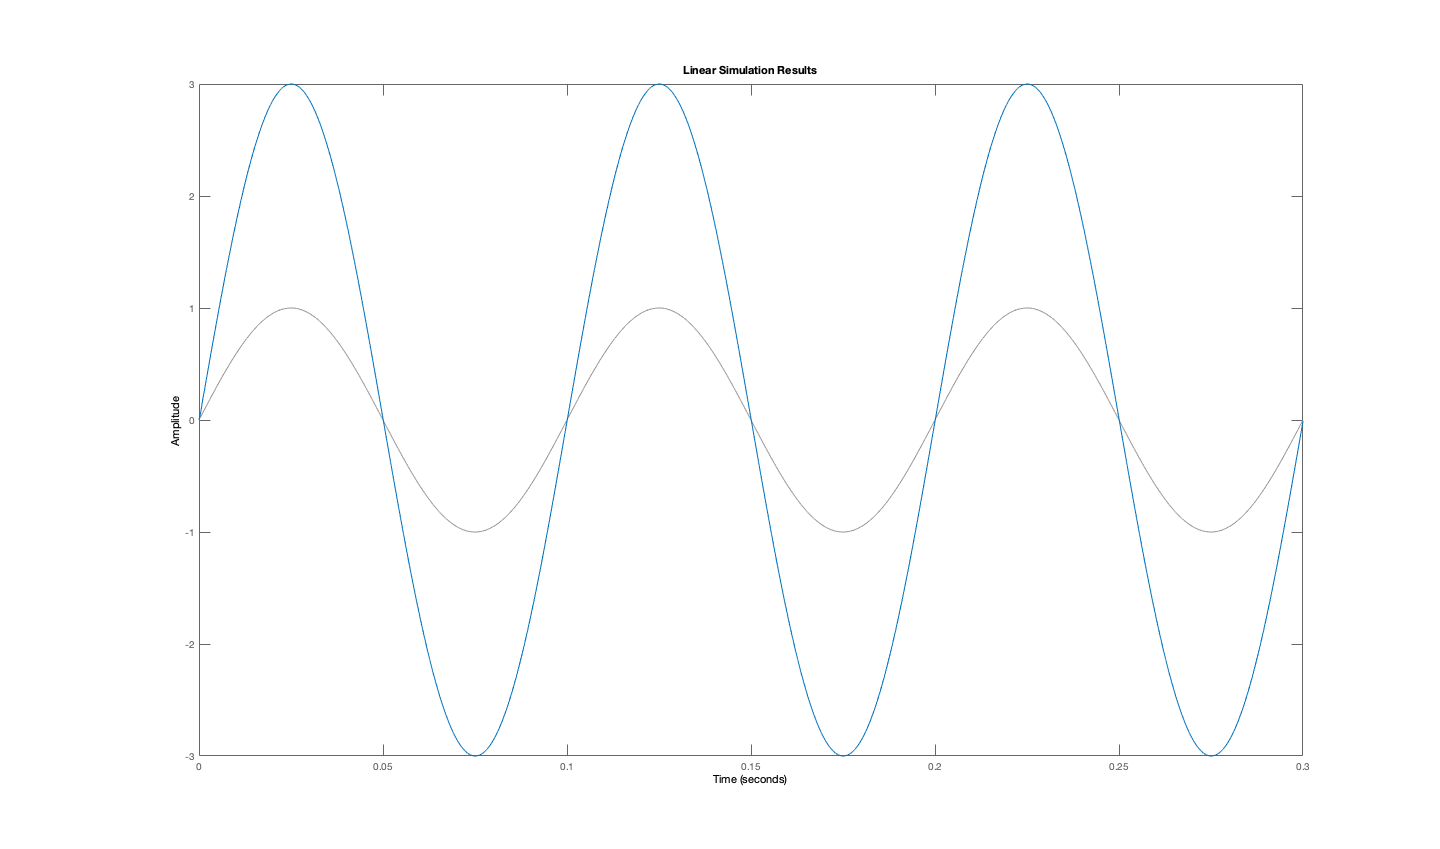
\includegraphics[width=8cm]{imagenes/rtasen10}	\caption{Respuesta a una señal senoidal de $10\Hz$}	
\end{figure}

Se observa que la señal representada con color azul es la salida  y el color gris es la señal de entrada. Notar la amplificacion a $3\V$ y que la señal no sufre atenuaci\'on visible, resultado esperable para esta frecuencia.\\

\begin{figure}[!h]
	\centering
	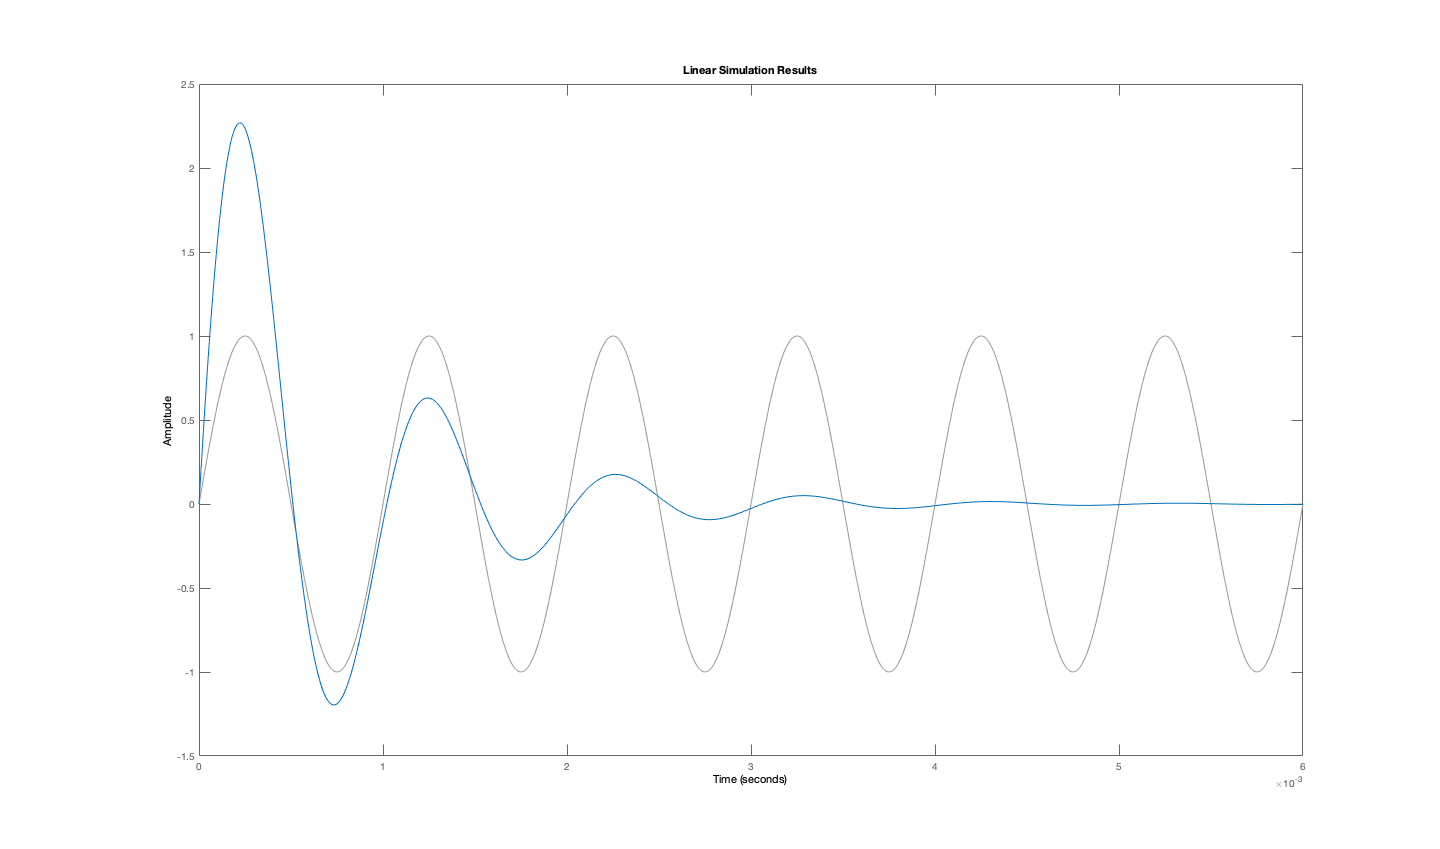
\includegraphics[width=8cm]{imagenes/rtasen1k}	\caption{Respuesta a una señal senoidal de $1\kHz$}	
\end{figure}

Aqui observamos que la salida sufre una gran atenuacion luego del transitorio, tanto que se puede considerar como de amplitud nula. Aqui se ve claramente el efecto de \textit{elimina-banda}, donde el filtro se encarga de que la señal no tenga amplitud apreciable si su frecuencia es de $1\kHz$.\\
Como ultimo comentario, la atenuaci\'on es total dado que la entrada es de tipo senoidal y estas funciones no estan compuestas por otras de distinta frecuencia,  como si es el  caso en señales triangulares o cudradas.\\

\begin{figure}[!h]
	\centering
	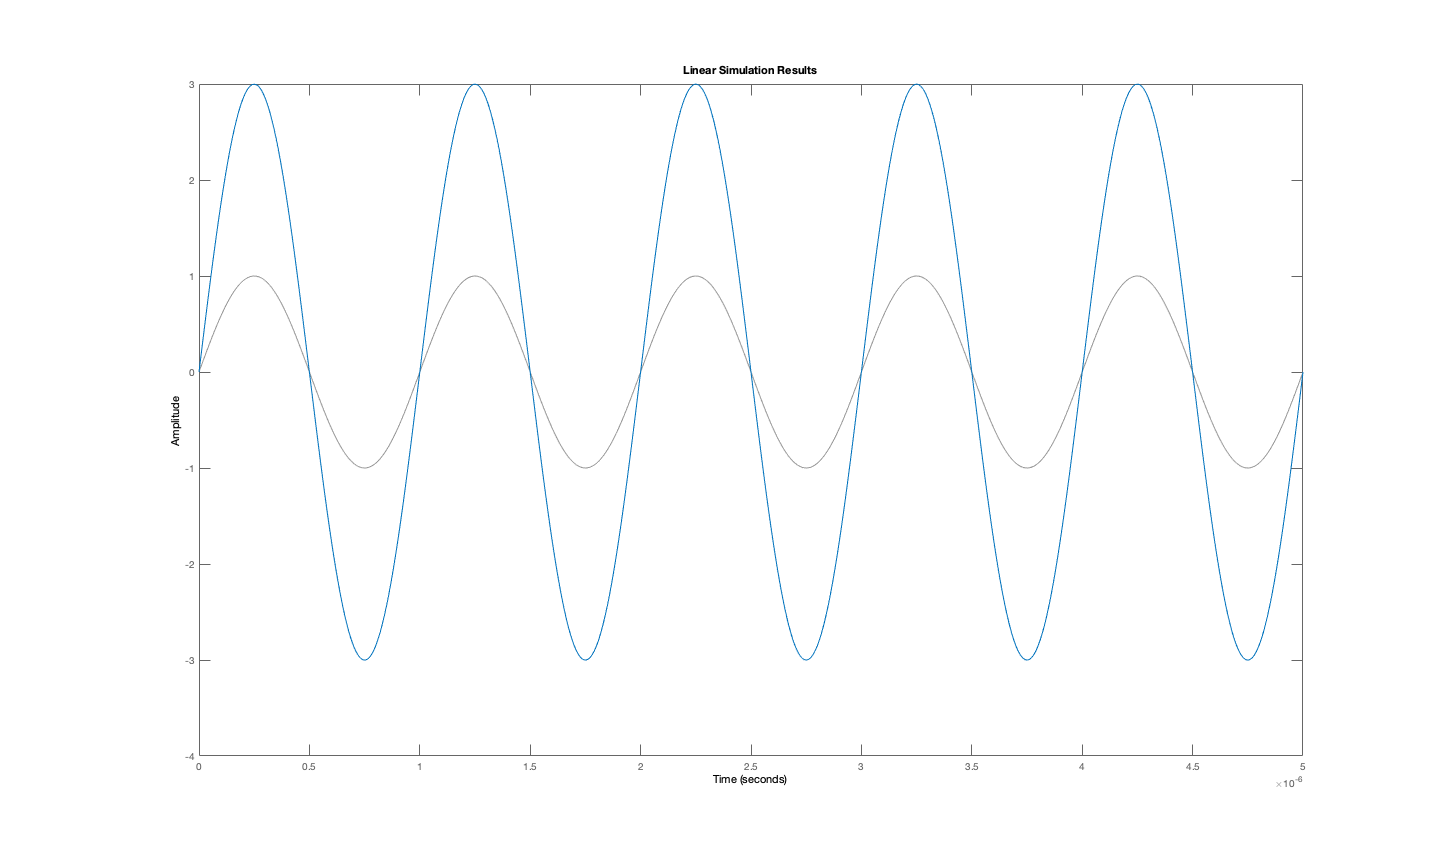
\includegraphics[width=8cm]{imagenes/rtasen100k}	\caption{Respuesta a una señal senoidal de $100\kHz$}	
\end{figure}
En esta respuesta, se ve un efecto similar a la respuesta a la senoidal de $10\Hz$, donde se ve un nivel de  amplificacion hasta los $3\V$ y la  señal no sufre atenuaci\'on visible.\\

\begin{figure}[hbt]
	\centering
	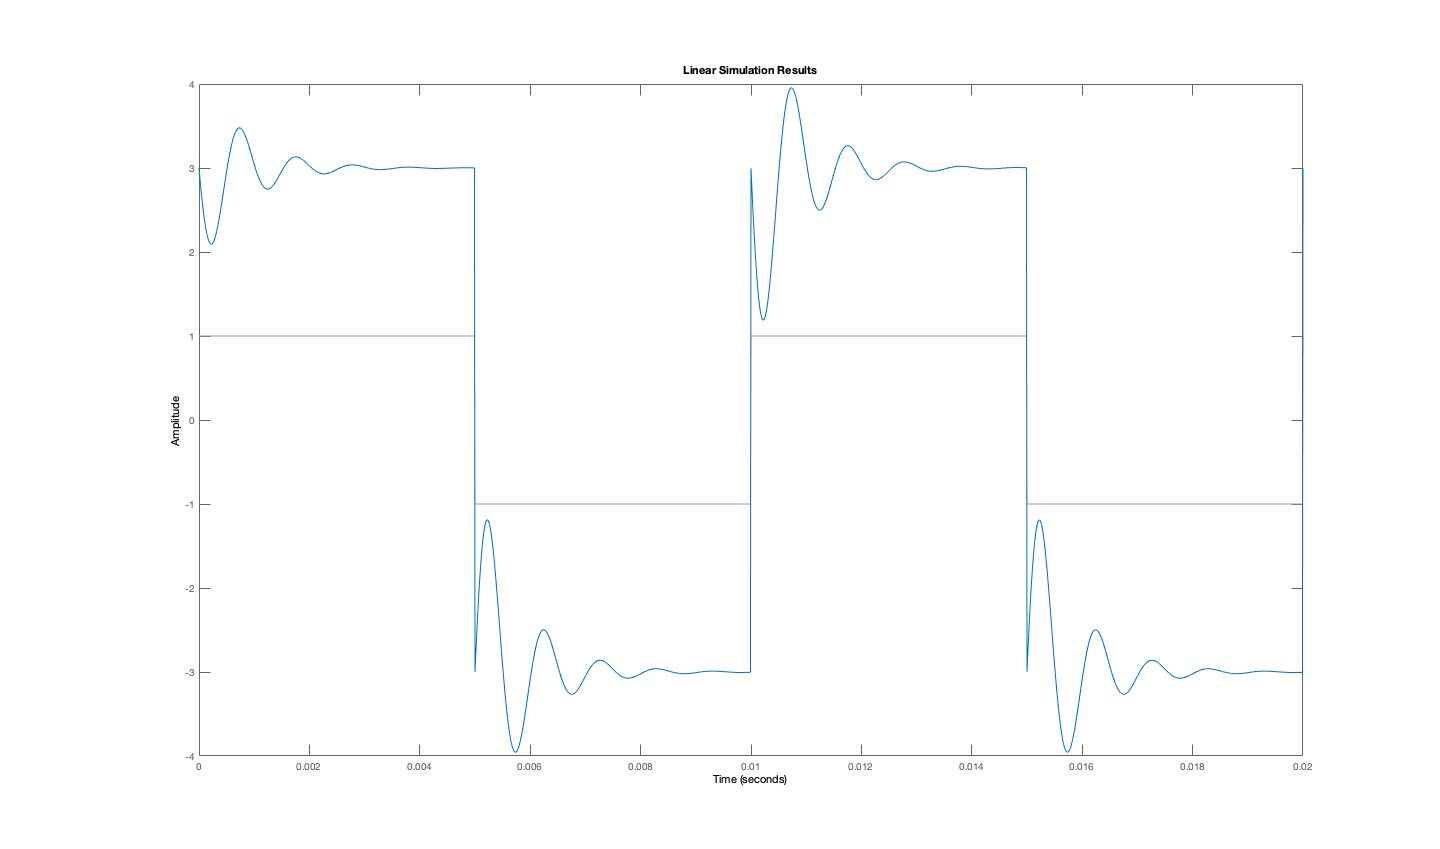
\includegraphics[width=8cm]{imagenes/rtasqar100}	\caption{Respuesta a una señal senoidal de $100\Hz$}	
\end{figure}

Se observa la salida a una señal cuadrada de $100 \Hz$, notar que el circuito responde muy similar al escal\'on, esto se debe a la baja frecuencia de esta señal, que tiene un per\'iodo mucho mas bajo que el tiempo caracteristico del circuito.

\begin{figure}[hbt]
	\centering
	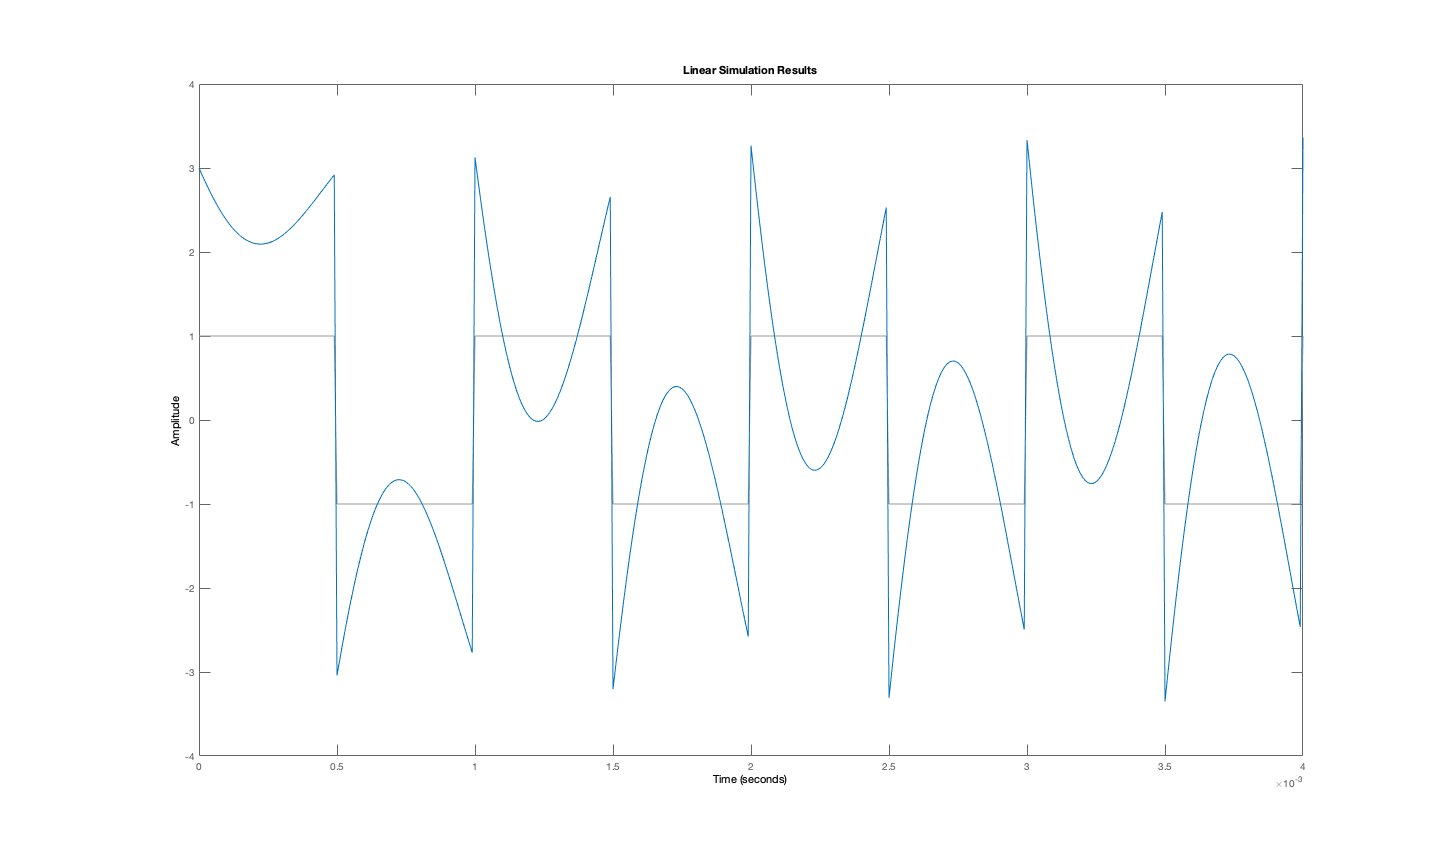
\includegraphics[width=8cm]{imagenes/rtasqar1k}	\caption{Respuesta a una señal senoidal de $1\kHz$}	
\end{figure}
En esta salida se observa una variaci\'on en la salida cada vez mas grande a medida que el tiempo avanza, con caracteristicas de oscilaci\'on muy predominantes.\\

\pagebreak
\begin{figure}[hbt]
	\centering
	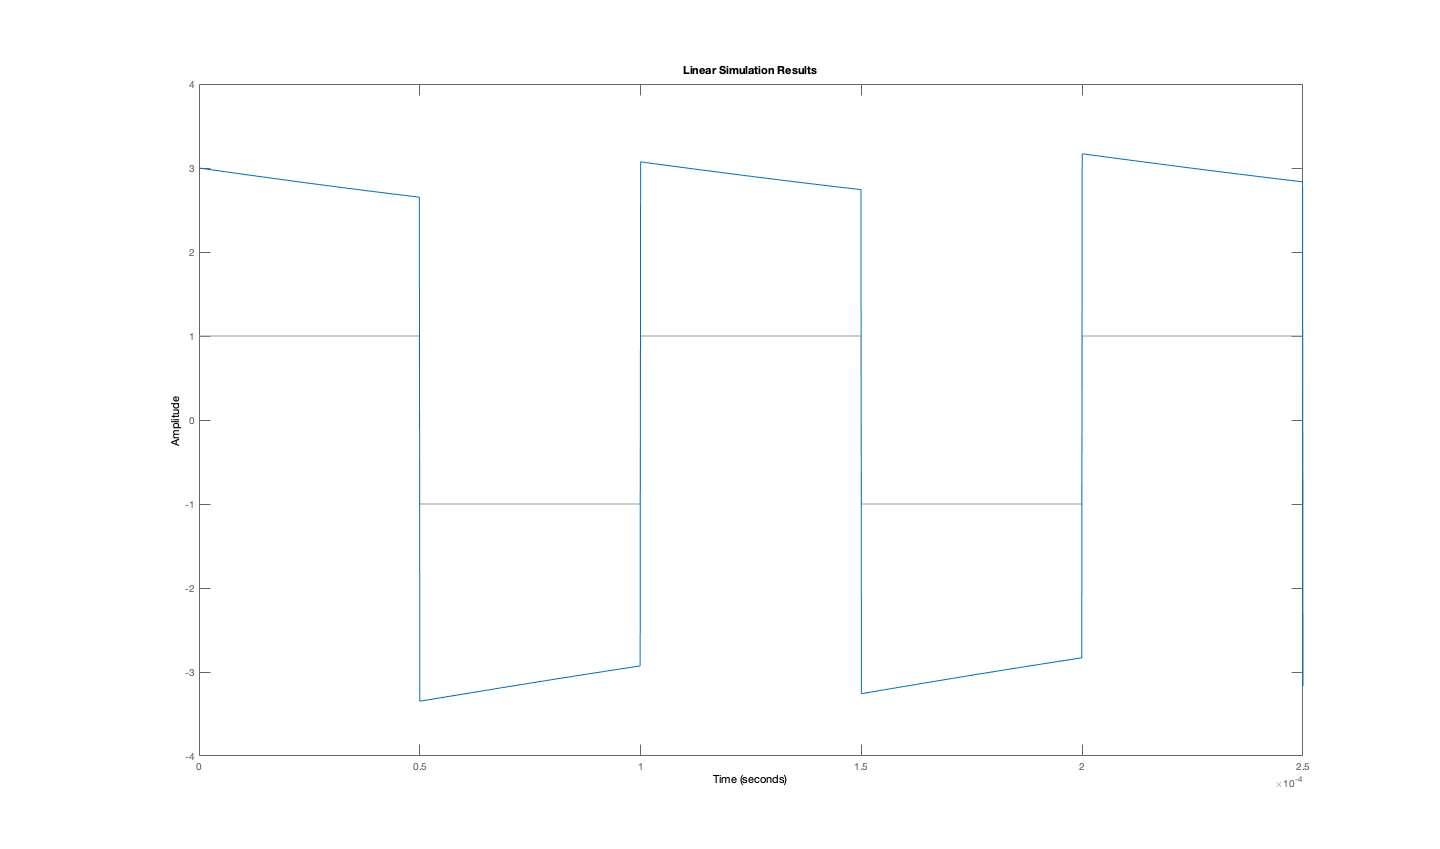
\includegraphics[width=8cm]{imagenes/rtasqar100k}	\caption{Respuesta a una señal senoidal de $100\kHz$}	
\end{figure}
Aqui se observa que la salida es menos oscilante que la anterior (sin considerar la  naturaleza oscilatoria de la señal de entada)
y que presenta una distorsion leve en cada semiciclo.

%---------------------------------------------------------------%

\subsection*{Simulaci\'on}
	Para verificar que el funcionamiento del circuito sea el esperado, se utiliz\'o el software de simulaci\'on \textit{LTSpice} con los componentes de valores comerciales. 
\begin{figure}[hbt]
	\centering
	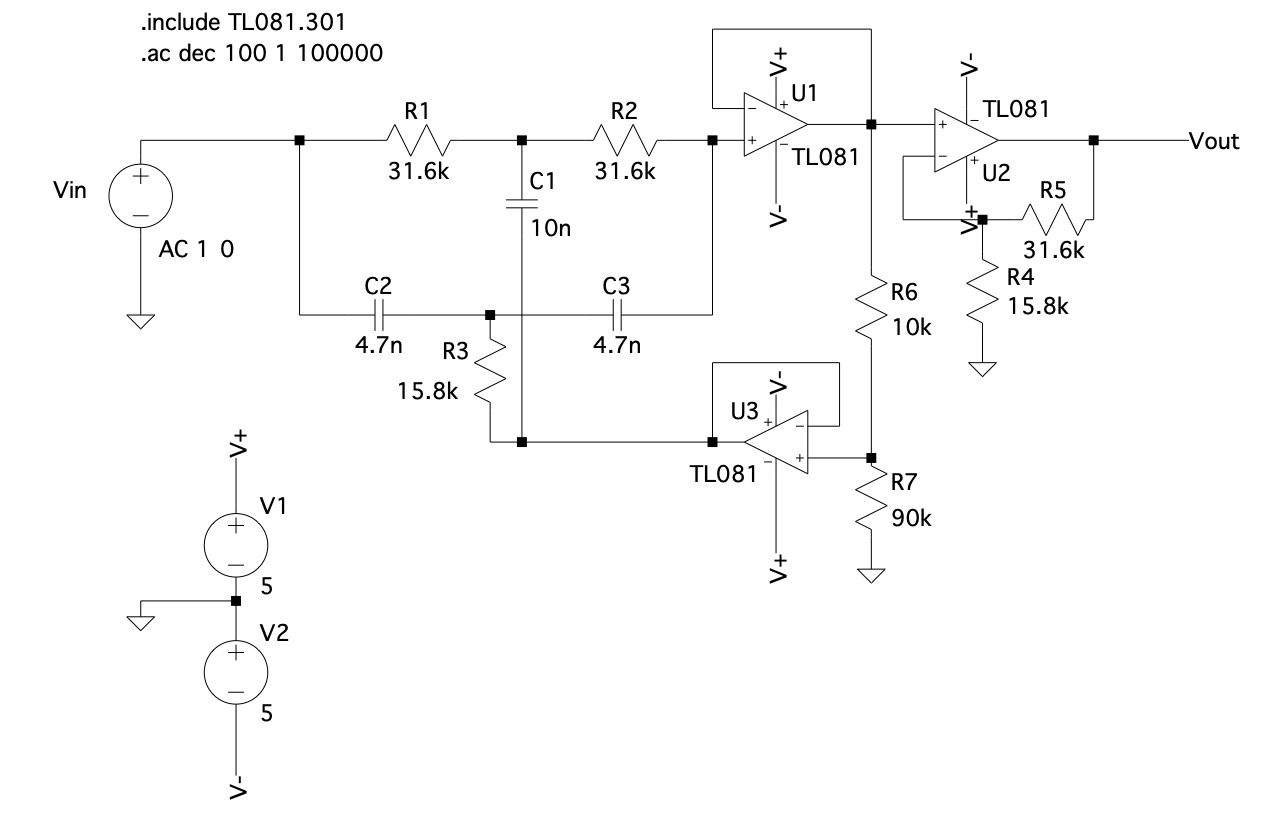
\includegraphics[width=10cm]{imagenes/simulacion}
	\caption{Circtuito simulado}
\end{figure}

	
Se utiliz\'o la directiva \texttt{.ac dec 100 1 1000000 } para
variar la  frecuencia de la fuente de entrada \texttt{ Vin } desde  $1 \si{\hertz}$ hasta $100 \kHz$. Luego se import\'o la biblioteca \textit{TL081} para el operacional. Produciendo el siguiente resultado.

%---------------------------------------------------------------%

\subsection*{Respuesta de la simulaci\'on a distintas señales}

%---------------------------------------------------------------%